\documentclass{article}

\usepackage{amsmath}
\usepackage{graphicx}

\begin{document}

\title{Homework 2: Multi-threading the Mandelbrot set}
\author{Geoffrey Ulman\\
        CSI702}
\date{February 2010}
\maketitle

\section{Background}

Benoit Mandelbrot plotted the first Mandelbrot set images in 1979 using an IBM mainframe as a means to understand the class of shapes discovered by Gaston Julia and Pierre Fatou and coined Julia sets\cite[p. 219]{chaos}. To plot a Julia set, one simply chooses a point c on the complex plane and applies the following simple iteration, plotting each point in the sequence:
\[ z \rightarrow z^2+c \]
The resulting shapes, when the iteration does not zoom off to infinity, form myriad patters: prickly branching sticks, curving nested shells, and islands arranged in complex spirals. To better understand the entire family of shapes, Mandelbrot imagined the set of points on the complex plane whose Julia sets are bounded. Mandelbrot's first computer printouts showed tantalizing hints at the infinitely varied structure of the set. However, taking advantage of the embarrassingly parallel nature of the set's definition with today's multi-core computers, we can generate truly breathtaking views into the seahorse valleys and ``devil's polymer'' of tiny filaments that run off in crazy patterns from the set's periphery\cite[p. 228]{chaos}.

\section{Design}

The output of both mandelbrot\_serial.c and mandelbrot\_threadded.c is an array containing the number of iterations required for the Julia set iteration to exit a circle of radius \(\sqrt{2}\) centered at the origin of the complex plane. This iteration is performed for discrete points evenly spaced on \( [-2,2] \) and \([-2i,2i]\). Points not exiting after 20000 iterations are assumed to be in the Mandelbrot set. Because the iterations for each point are independent from one another, the problem is highly parallel. Also, because absolutely no cooperation is needed between threads performing iterations for different regions of the complex plane, no sophisticated synchronization (using mechanisms like mutexes) is required.

My multi-threaded design creates \(n\) threads which evenly divide rows of the Mandelbrot set among themselves. Many of these threads finish very quickly because many Julia sets for points near the array edges diverge almost immediately. With enough threads, however, the work is partitioned finely enough that four cores are easily kept busy throughout the entire computation. The hypothesis which motivated this design was that the performance penalty for starting many threads would be small relative to the computations to be performed. Further, I believe that the resulting code is cleaner and more readable than a more complicated approach would allow.

My decision to portion sections of work among the threads by row (instead of in some smaller increment which might have more evenly balanced the load among the threads) was motivated by two factors. First, giving each thread a consecutive block of rows meant that each thread would be responsible for filling in a block of consecutive values in memory. Theoretically, this spatial locality could improve the efficiency of the code's memory writes. Second, it was a simple approach which resulted in clean and readable code.

\section{Performance}

We have three basic methods available for profiling c code: the UNIX time command, the c clock() function, and gprof. Because we are profiling multi-threaded code, which method to use must be carefully considered. The c clock() library function returns ``the processor time used by the program since the beginning of execution, or -1 if unavailable''\cite[p.255]{cpl}. Thus, placing clock() calls at the beginning and end of main() results in a time roughly equivalent to the ``user'' time reported by the UNIX time command---which measures, according to the time man page, the ``total number of CPU-seconds that the process used directly (in user mode), in seconds.'' Therefore, both these methods are misleading because they count time spent on each core. We would expect the results to be essentially the same for both the parallel and threaded codes.

Profile results from gprof are also potentially misleading. It does not appear to be thread-aware, outputting timing only for the main thread of execution. Finally, the ``sys'' value reported by UNIX time is not helpful, since we want to measure the amount of effort required to perform the Julia set iterations, whereas ``sys'' only reports on time spent by the process in ``kernel-mode'' (performing system calls, file io, etc\ldots). Therefore, we are left with the ``real'' value reported by UNIX time. This does have the disadvantage of potentially being affected by other processes running on the system, but by running many runs and observing general trends, this effect can be minimized.

I ran a series of experiments modifying the size of the Mandelbrot image array (\(n\)) and the maximum number of Julia set iterations (\(itmax\)). The following figures show total clock time for both the serial and parallel codes as well as the speedup multiplier achieved by the parallel code. Each figure fixes the maximum number of Julia set iterations and varies the size of the Mandelbrot image array. All experiments were run using a Dell Precision M4400 laptop with two Intel Core2 Extreme CPU Q9300 @ 2.53GHz processors for a total of four cores. Thus, we do not expect to be able to do better than a four times speedup with parallelization alone.

\begin{figure}
\centering
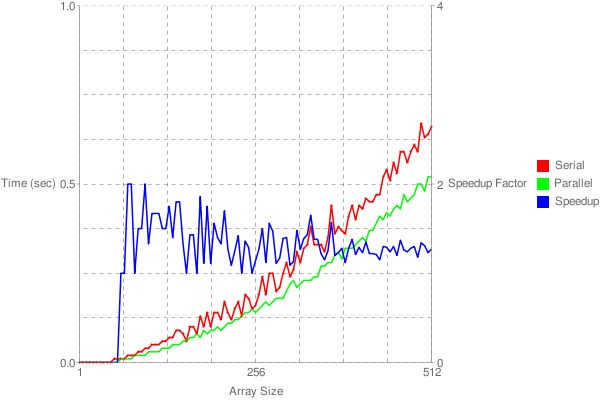
\includegraphics[width=0.9\textwidth]{chart1nt.png}
\caption{1 to 512 Array Size---2000 Maximum Julia Set Iterations}
\label{chart1}
\end{figure}

\begin{figure}
\centering
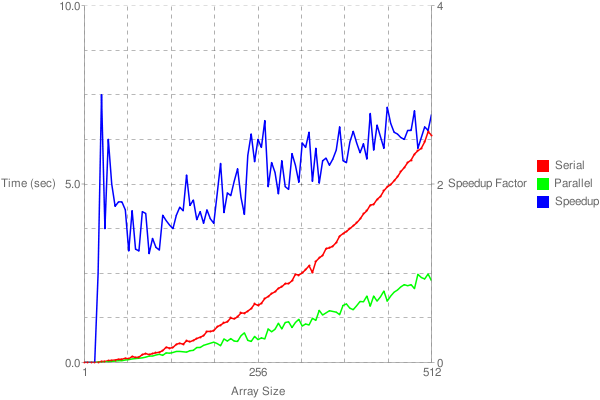
\includegraphics[width=0.9\textwidth]{chart2nt.png}
\caption{1 to 512 Array Size---20000 Maximum Julia Set Iterations}
\label{chart2}
\end{figure}

For the relatively small \(n\) and \(itmax\) values used in Figure \ref{chart1} and Figure \ref{chart2}, both the serial and parallel codes complete quickly enough that the thread creation and disposal overhead almost overwhelms the advantage of the parallel code. The average speedup attained in Figure \ref{chart1} was approximately 1.35 times. The average speedup attained in Figure \ref{chart2} was approximately 2.10 times. While they do represent an improvement, neither of these values is very impressive considering four cores were available to the code.

\begin{figure}
\centering
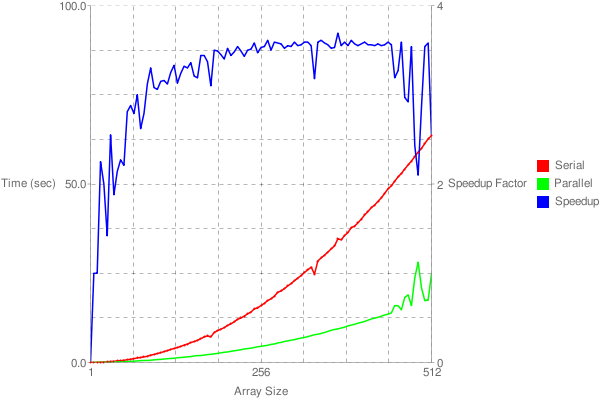
\includegraphics[width=0.9\textwidth]{chart3nt.png}
\caption{1 to 512 Array Size---200000 Maximum Julia Set Iterations}
\label{chart3}
\end{figure}

With \(itmax = 200000\) and \(n > 256\) the parallel code appears to reach it's maximum performance with an average speedup of approximately 3.49 times. Figure \ref{chart3} clearly shows this plateau. However, there also appears to be signs of trouble. The speedup of some runs with \(n\) near 512 fall well short of the maximum observed speedup. It was not clear from the results shown in Figure \ref{chart3} whether this was a real phenomenon, or whether it was caused by external factors.

\begin{figure}
\centering
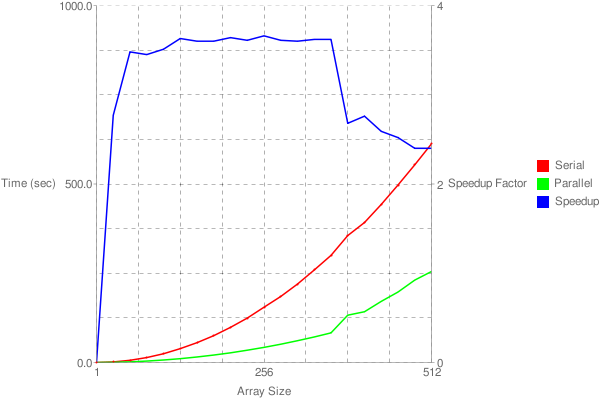
\includegraphics[width=0.9\textwidth]{chart4nt.png}
\caption{1 to 512 Array Size---2000000 Maximum Julia Set Iterations}
\label{chart4}
\end{figure}

Figure \ref{chart4} more clearly demonstrates this drop off. As the runs get longer, the advantage enjoyed by the parallel code clearly drops off. This cannot be attributed to memory issues, as only \(itmax\) varied between Figure \ref{chart3} and Figure \ref{chart4}. My hypothesis is that the longer runs were interrupted more often by periodic operating system tasks which the shorter runs did not encounter.

Finally, to more fully explore the effect of modifying \(n\), a last experiment was run with much larger Mandelbrot image array sizes than the previous trials. The results, shown in Figure \ref{chart5}, are strikingly similar to Figure \ref{chart4}. Regardless of whether the execution time is long because of large \(n\) or large \(itmax\), the performance gain appears to decrease for runs lasting longer than 400 to 500 seconds. I did attempt to increase the process priority using the UNIX nice command, but the results were similar.

I also hypothesized that perhaps creating so many threads was causing performance problems (perhaps there was excessive overhead from contex switches---swapping threads on and off the CPU). Although this theory was somewhat contradicted by the results from Figure \ref{chart4} which show poor performance for less than 512 threads, I decided to test it by creating an alternative threaded code which creates a small number of threads that are not assigned sections of the Mandelbrot array statically. Instead, they get rows of the array to process dynamically by checking the value of a global int variable which indicates the next unprocessed row. Mutually exclusive access to the global variable is controlled by a mutex. However, I observed a similar performance degradation with this code. This left me with my original hypothesis, that other periodic system processes were degrading the performance of long multi-threaded runs.

\begin{figure}
\centering
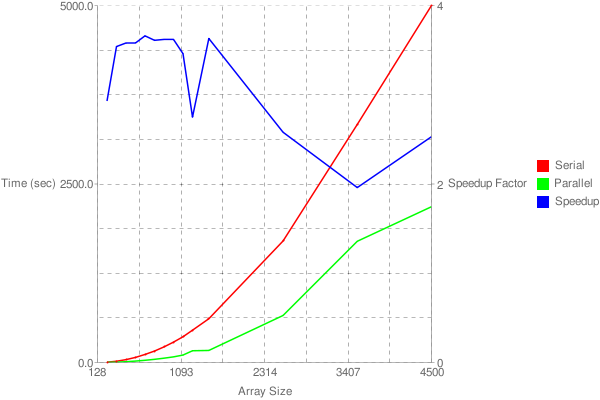
\includegraphics[width=0.9\textwidth]{chart5nt.png}
\caption{500 to 4500 Array Size---200000 Maximum Julia Set Iterations}
\label{chart5}
\end{figure}

\section{Conclusion}
My straightforward multi-threaded design was able to achieve a 3.5 times speedup over the serial code under optimal circumstances on a four core machine. This performance did not scale to runs lasting longer than 400 to 500 seconds, but even in those poor cases a 2.5 times speedup was always achieved. I believe that on a dedicated server the performance for longer runs would improve. 

\begin{thebibliography}{9}

\bibitem{chaos}
  James Gleick,
  \emph{Chaos: Making A New Science},
  Penguin Books, New York,
  1988.

\bibitem{cpl}
  Brian W. Kernighan and Dennis M. Ritchie,
  \emph{The C Programming Language},
  Prentice Hall PTR, New Jersey,
  2009.

\end{thebibliography}

\end{document}
